\section{Highest Locker Priority}

\subsection{Definition}

Highest Locker Priority (HLP) is the improvement of the previous protocol to allow the highest priority task $\tau_{i}$ that doesn't use resource $R_{k}$ to interrupt the lower priority task $\tau_{j}$ that use the resource, $R_{k}$ by limiting the raised priority of the task $\tau_{j}$. So, 
 
\begin{center}
 $p_{j}(R_{k})=\underset{h}{\mathrm{max}} \{P_{h}| \tau_{h}$ uses $R_{k}\}  $ \cite{b5}
\end{center}

whereas the priority of task, $\tau_{j}$ that are currently accessing the resource, $R_{k}$ in increased to the maximum only among the taskThis dynamic priority then set back to its nominal value $P_{i}$ when the task leave its critical section. The maximum raised priority of a task $\tau_{j}$ is called priority ceiling $ C(R_{k}) $ and computed off-line.  The maximum priority $ C(R_{k}) $ of the tasks sharing $ R_{k} $ is the computed online such

\begin{center}
$C(R_{k})\stackrel{def}{=}\underset{h}{\mathrm{max}} \{P_{h}| \tau_{h}$ uses $R_{k}\}  $ \cite{b5}
\end{center}

Since the priority of lower priority task $\tau_{j}$ is raised as soon as the task entering $ R_{k} $, this protocol also known as Immediate Priority Ceiling. This protocol can be visualize as in figure \ref{fig: Example_of_schedule_under_HLP} where task $ \tau_{1} $ have higest priority and task $ \tau_{3} $ is the first task arrive

\begin{figure}[h]
    \centering
    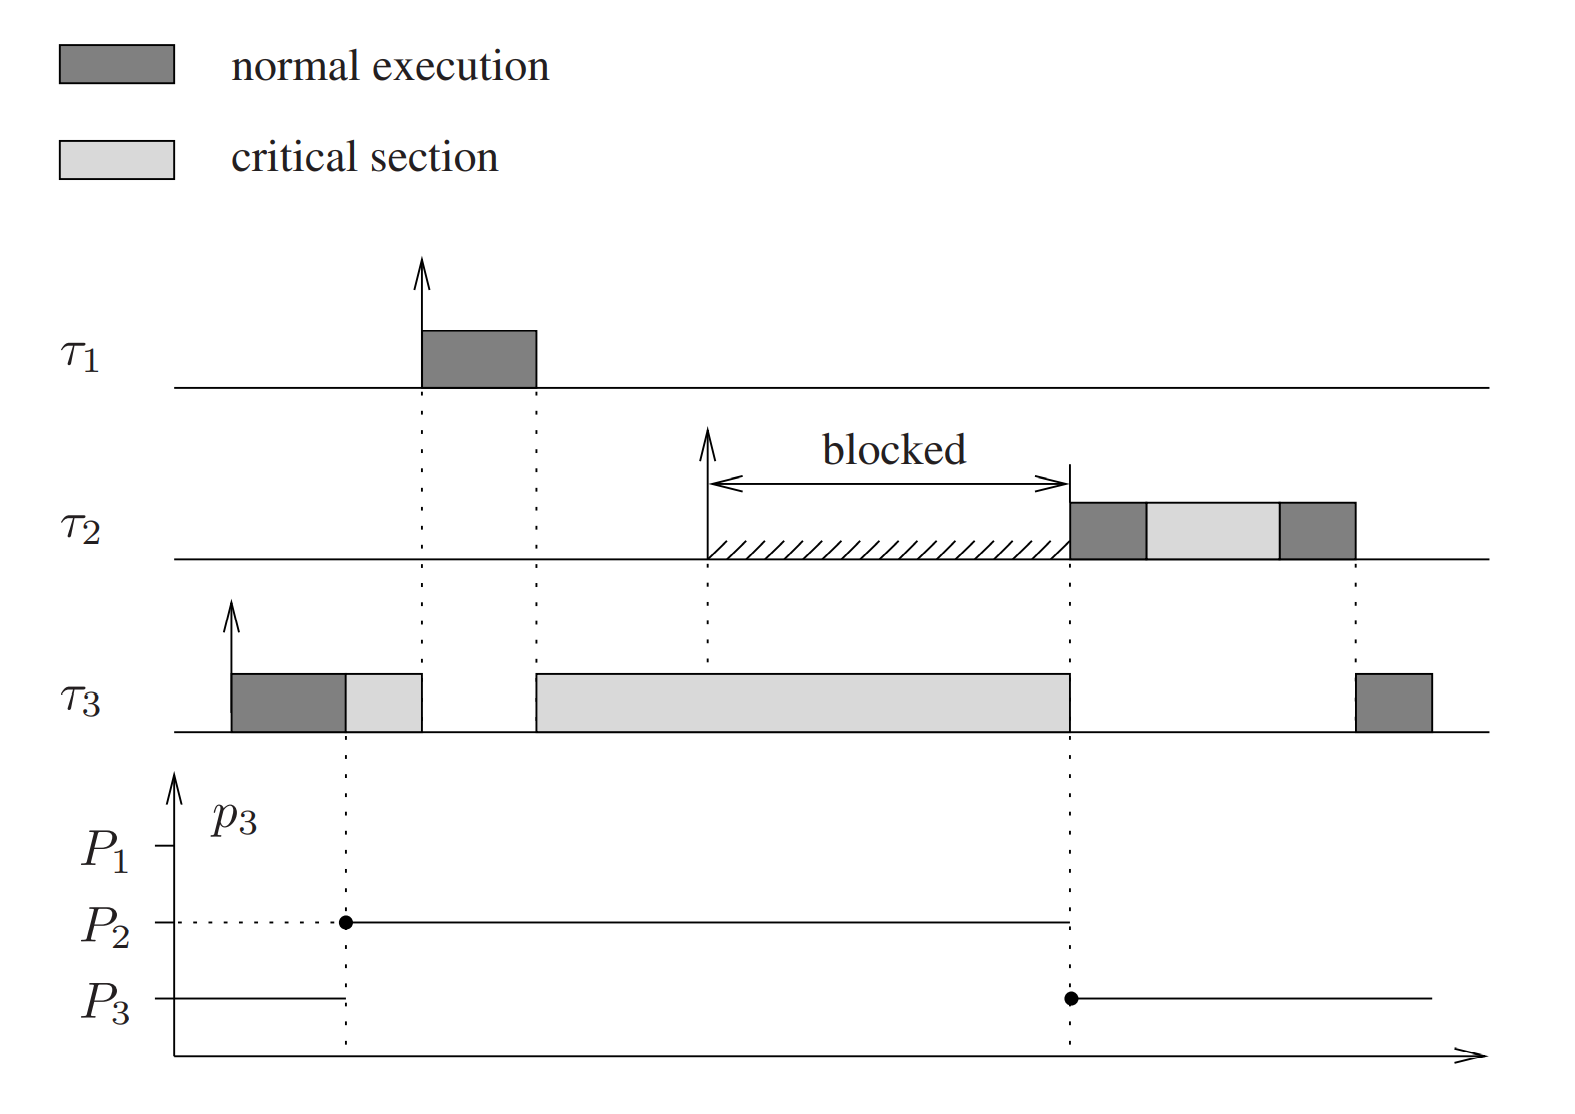
\includegraphics[width=0.5\textwidth]{Example_of_schedule_under_HLP}
    \caption{ Example of schedule under HLP, where $ p3 $ is raised at the level $ C(R) = P_{2} $ as soon as $ \tau_{3} $ starts using resource R \cite{b5}}
    \label{fig:Example_of_schedule_under_HLP}
\end{figure}

 
\subsection{Blocking Time Computation}

So, total of critical section of lower priority task $\tau_{j}$ blocking higher priority task $\tau_{i}$ is reduced by adding new parameter as shown below.

\begin{center}
$ \gamma_{i}=\{Z_{j,k} | P_{j}<P_{i} $ and $ C(R_{k})\geq P_{i} \} $ \cite{b5}
\end{center}

According to \cite{b5} - Under HLP, a task $ \tau_{i} $ can be blocked, at most, for the duration of a single critical section belonging to the set $ \gamma_{i} $ and this theorem is proved by contradiction,  

Below is the proof of the theorem according to \cite{b5}.

Assuming that $ \tau_{i} $ is blocked by two critical sections, $ z_{1,a} $ and $ z_{2,b} $. 
For this to happen, both critical sections must belong to different tasks ($ \tau_{1} $ and $ \tau_{2} $) with priority lower than $ P_{i} $, and both must have a ceiling higher than or equal to $ P_{i} $. That is, by assumption, we must have

\begin{center}
$ P_{1}< P_{i}\leq C(R_{a})$

$ P_{2}< P_{i}\leq C(R_{b})$
\end{center}

Now, $ \tau_{i} $  can be blocked twice only if $ \tau_{1} $  and $ \tau_{2} $  are both inside the resources when $ \tau_{i} $ arrives, and this can occur only if one of them (say $ \tau_{1} $ ) preempted the other inside the critical section. But, if $ \tau_{1} $  preempted $ \tau_{2} $ inside $ z_{2,b} $  it means that $ P_{2}> C(R_{b}) $ , which is a contradiction. Hence, the theorem follows.

As shown in figure \ref{fig:Example_of_schedule_under_HLP}, $ \tau_{i} $ can be block at maximum once, means that

\begin{center}
$B_{i}(R_{k})=\underset{j,k}{\mathrm{max}} \{ \delta_{j,k}-1 | Z_{j,k} \in \gamma_{i}\}  $ \cite{b5}
\end{center}

We need to minus one unit of time because the lower priority task $ \tau_{j} $ need to access $ R_{k} $ atleast one unit time earlier then $ \tau_{i} $ to block it.

\subsection{Implementation Strategies} 

According to \cite{b6} - Fewer RTOSs support the Highest Locker Pattern more than the basic Priority Inheritance Pattern. The implementation of this pattern  is fairly straightforward, with the addition of priority ceiling attributes in the Shared Resource. When the mutex is locked, it must notify the Scheduler to elevate the priority of the locking task to that resource's priority ceiling.

\subsection{Sample Model} 

The following example model is totally taken from \cite{b6}.

In the example shown in Figure \ref{fig:hlp_model}, there are four tasks with their priorities shown using constraints, two of which, Waveform Draw and Message Display, share a common resource, Display. The tasks, represented as active objects in order of their priority, are Message Display (priority Low), Switch Monitor (priority Medium Low), Waveform Draw (priority Medium High), and Safety Monitor (priority Very High), leaving priority High unused at the outset. Message Display and Waveform Draw share Display, so the priority ceiling of Display is just above Waveform Draw (that is, High). 

The scenario runs as follows: First, the lowest-priority task, Message Display, runs, calling the operation Display.displayMsg(). Because the Display has a mutex semaphore, this locks the resource, and the Scheduler (not shown in Figure 7-11) escalates the priority of the locking task, Message Display, to the priority ceiling of the resource—that is, the value High.
 
While this operation executes, first the Switch Monitor and then the Waveform Draw tasks both become ready to run but cannot because the Message Display task is running at a higher priority than either of them. The Safety Monitor task becomes ready to run. Because it runs at a priority Very High, it can, and does, preempt the Message Display task. 

After the Safety Monitor task returns control to the Scheduler, the Scheduler continues the execution of the Message Display task. Once it releases the resource, the mutex signals the Scheduler, and the latter  225 deescalates the priority of the Message Display task to its nominal priority level of Low. At this point, there are two tasks of a higher priority waiting to run, so the higher-priority waiting task (Waveform Draw) runs, and when it completes, the remaining higher-priority task (Switch Monitor) runs. When this last task completes, the Message Display task can finally resume its work and complete.

\begin{figure}[h]
    \centering
    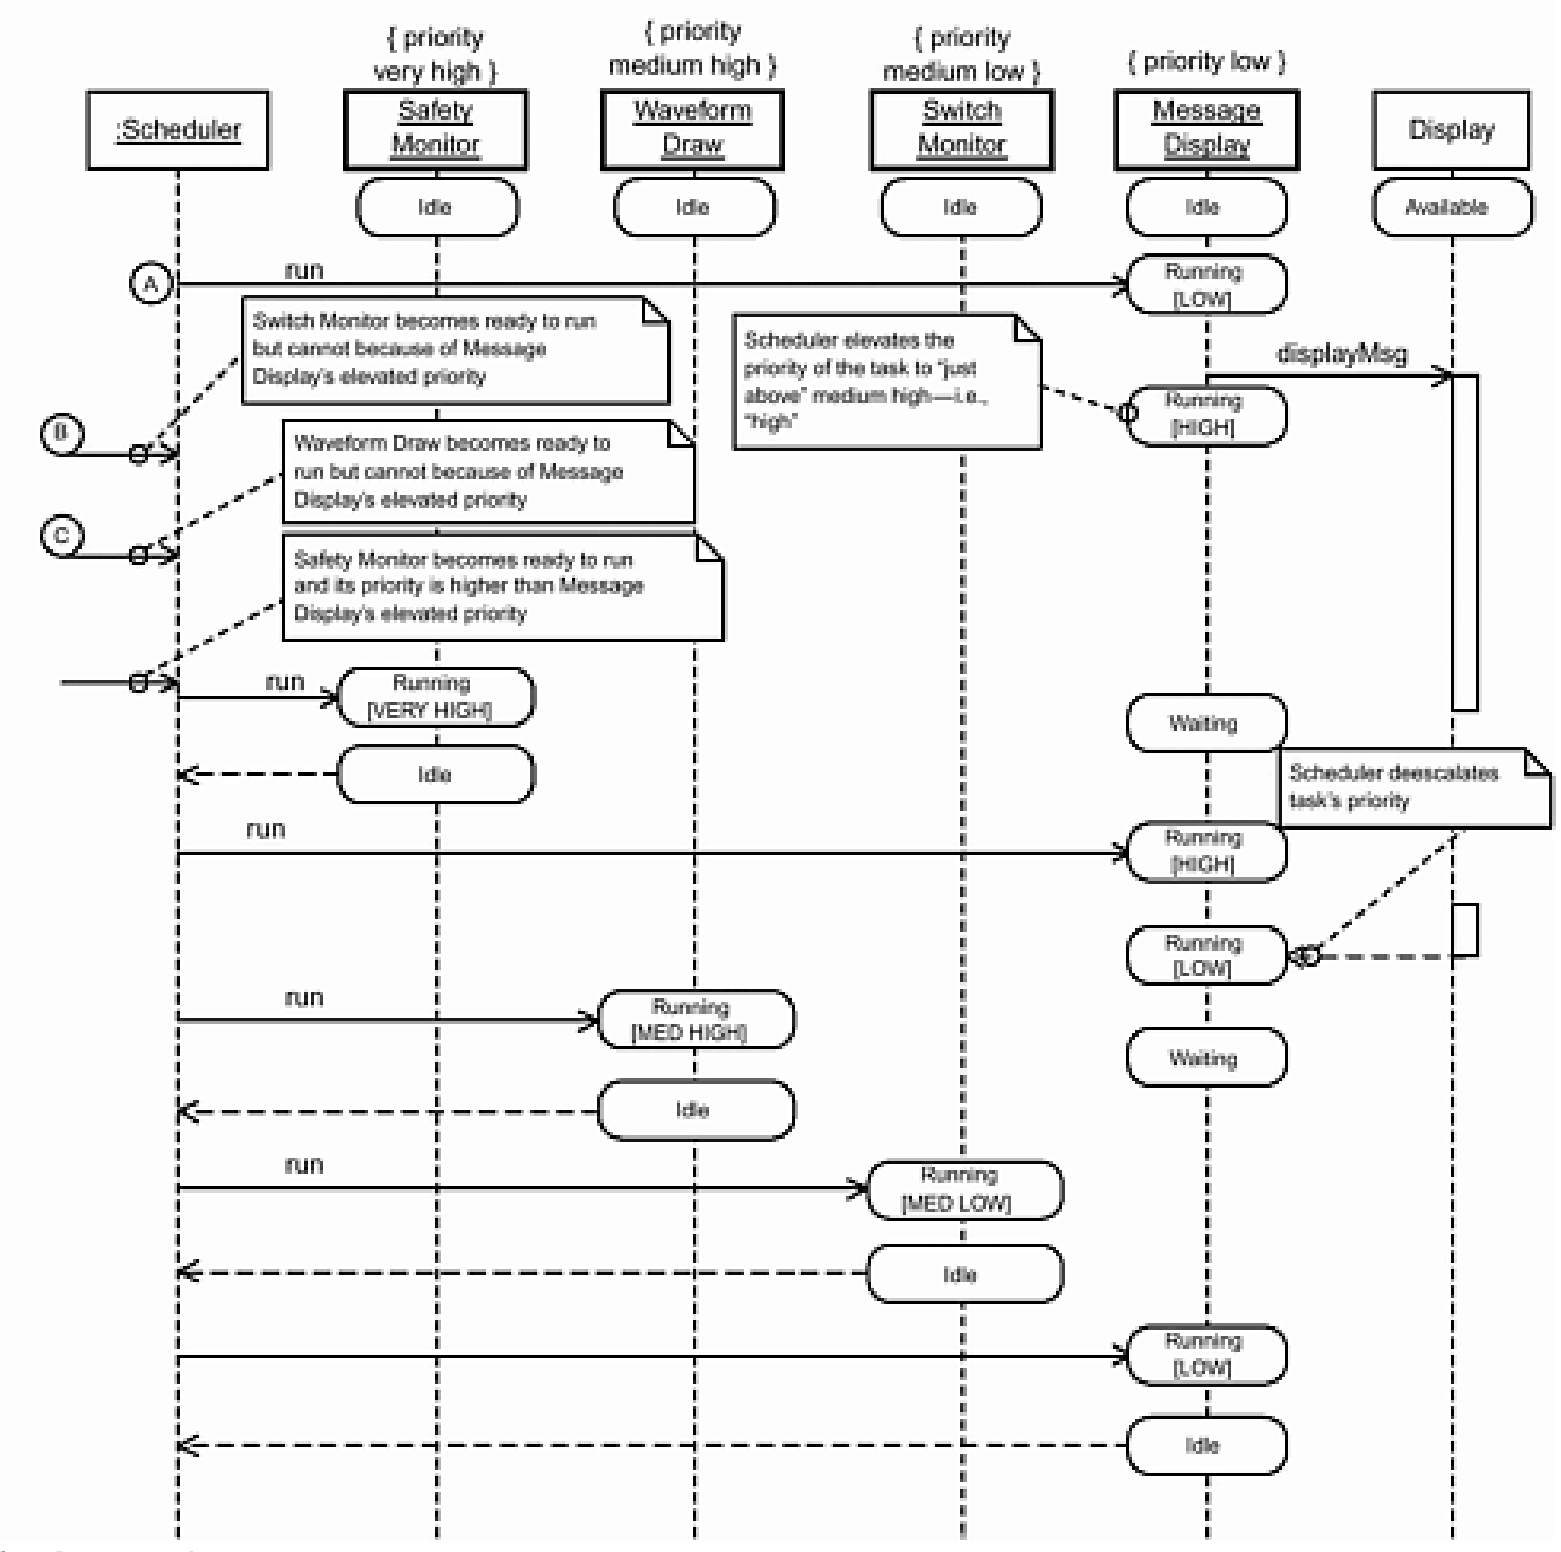
\includegraphics[width=0.5\textwidth]{hlp_model}
    \caption{ Example of schedule under HLP \cite{b6}}
    \label{fig:hlp_model}
\end{figure}


\subsection{Problem Arise}

As claimed by \cite{b5}, despite the fact that this algorithm improve the previous algorithm, it still could produce some unnecessary blocking. This algorithm block a task at the time it attempt, before it actually require a resource \cite{b5}. It also says that - If a critical section is contained only in one branch of a conditional statement, then the task could be unnecessarily blocked, since during execution it could take the branch without the resource.

Another downside of this protocol according to \cite{b6} is that the deadlock could happen if a task that is currently accessing a mutually exclusive resource suspends it self.
 










